\capitulo{5}{Aspectos relevantes del desarrollo del proyecto}

%Este apartado pretende recoger los aspectos más interesantes del desarrollo del proyecto, comentados por los autores del mismo.
%Debe incluir desde la exposición del ciclo de vida utilizado, hasta los detalles de mayor relevancia de las fases de análisis, diseño e implementación.
%Se busca que no sea una mera operación de copiar y pegar diagramas y extractos del código fuente, sino que realmente se justifiquen los caminos de solución que se han tomado, especialmente aquellos que no sean triviales.
%Puede ser el lugar más adecuado para documentar los aspectos más interesantes del diseño y de la implementación, con un mayor hincapié en aspectos tales como el tipo de arquitectura elegido, los índices de las tablas de la base de datos, normalización y desnormalización, distribución en ficheros3, reglas de negocio dentro de las bases de datos (EDVHV GH GDWRV DFWLYDV), aspectos de desarrollo relacionados con el WWW...
%Este apartado, debe convertirse en el resumen de la experiencia práctica del proyecto, y por sí mismo justifica que la memoria se convierta en un documento útil, fuente de referencia para los autores, los tutores y futuros alumnos.


\section{Elección del lenguaje de programación}\label{EleccionLenguaje}

Spark es un sistema que proporciona soporte a diferentes lenguajes de programación: Java, Scala, Python y, recientemente, R~\cite{SparkDoc}. Eliminando este último como posible elección, por el desconocimiento del lenguaje y la poca documentación que hay sobre su uso con Spark, se ha realizado una comparativa entre las opciones restantes que podrían seleccionarse para llevar a cabo el proyecto.

Para elegir los aspectos a tener en cuenta durante esta comparación me he basado en el estándar ISO 9126 para la calidad del software~\cite{ISO9126}. Los puntos a analizar han sido finalmente los siguientes: \\

\begin{itemize}
	\item \textbf{Experiencia previa:} Se tendrá en cuenta el contacto que se haya tenido con los lenguajes anteriormente.
	\item \textbf{Eficiencia de ejecución:} Valoraremos el rendimiento de cada lenguaje en función del tiempo que requieren para la ejecución de programas. 
	\item \textbf{Facilidad de mantenimiento:}  Las ventajas y facilidades del lenguaje en el caso de que se requiriese corregir o mantener un algoritmo o aplicación. 
	\item \textbf{Adecuación:} Beneficios aportados por el lenguaje para su uso concreto en el desarrollo de algoritmos para Spark.
	\item \textbf{Documentación disponible:} Facilidad para encontrar información actualizada sobre el uso del lenguaje en Spark.
	
\end{itemize}

Nótese que la tabla \ref{tabla:ComparativaJavaScalaPython} es una comparativa entre las características de los diferentes lenguajes para su uso en Spark, no una comparativa entre las características propias de cada uno. Por lo tanto, aspectos que no tengan influencia en Spark o aquellos que sean iguales para todos los lenguajes, como, por ejemplo, la portabilidad, no serán incluidos en la comparativa. Así mismo, si dos lenguajes compartiesen una característica muy parecida o idéntica, esta será incluida una sola vez en la comparativa, fusionando las dos celdas que correspondan de la tabla \ref{tabla:ComparativaJavaScalaPython}.

\tablaApaisadaSmall{Comparativa entre características de Java, Scala y Python para trabajar sobre Spark.}{m{2.65cm} m{5.3cm} m{5.3cm} m{5.3cm}}{ComparativaJavaScalaPython}
{\centering Criterio & \centering Java & \centering Scala  & \multicolumn{1}{c}{Python} \\}{

\centering Experiencia previa & Se ha trabajado en Java múltiples veces durante el grado. & Es un lenguaje sobre el que nunca se ha trabajado. & Se han aprendido las nociones básicas durante la carrera. \\ [0.2cm]


\centering Eficiencia de ejecución & \multicolumn{2}{m{11.05cm}}{Compila los ficheros generando archivos .class y los ejecuta sobre una máquina virtual de Java (JVM). Esto conlleva que la ejecución sea considerablemente más rápida que la del intérprete de Python.} & Es un lenguaje interpretado, lo que afecta negativamente a su rendimiento. Sin embargo, su rendimiento en comparación con Scala mejora considerablemente si contamos con muchos procesadores~\cite{PythonVsScala}.  \\ [0.2cm]


\centering Facilidad de mantenimiento & Código más extenso, aunque la aparición Java 8, con elementos como las funciones lambda (ver \ref{subsec:ExplLambdaJava}), han mejorado este aspecto. & \multicolumn{2}{m{11.05cm}}{Menos líneas de código y una sintaxis más fácilmente legible.} \\ [0.2cm]

\centering Adecuación & Trabajar sobre Java nos obliga, a la hora de programar, a transformar estructuras y clases de Spark solo soportadas al trabajar en Scala o Python. Además, no cuenta con un intérprete interactivo. & \multicolumn{2}{m{11.05cm}}{Spark está pensado para trabajar sobre Scala o Python. De hecho, Spark ha sido creado en Scala, por lo que su conocimiento puede ayudar a lo largo del proyecto. Ambos lenguajes cuentan con un intérprete interactivo. } \\ [0.2cm]

\centering Documentación disponible & Existe buena documentación en la página oficial de Spark, aunque es más escasa en otras fuentes. Además, muchas veces la documentación no trabaja sobre Java 8. & \multicolumn{2}{m{11.05cm}}{Existe una amplia documentación sobre el uso de ambos lenguajes en Spark.} \\ [0.2cm]
} 

\newpage


La elección final del lenguaje a utilizar será Scala, argumentando lo siguiente sobre los puntos que hemos comparado:

\begin{itemize}
	\item \textbf{Sobre la experiencia previa:} No se considera un problema aprender el lenguaje. Además, los archivos generados tras la compilación y, por consiguiente, la manera de ejecutarlos o monitorizar su rendimiento, es similar a Java, un lenguaje ya conocido.
	\item \textbf{Sobre la eficiencia de ejecución:} El rendimiento, en lo que a tiempo de ejecución se refiere, es muy similar a Java, por lo que se considera una ventaja frente Python.
	\item \textbf{Sobre la facilidad de mantenimiento:} En el momento de la elección del lenguaje no contamos con experiencia en el mantenimiento de un gran código de minería de datos, pero parece lógico que a menos cantidad de líneas que mantener, más fácil puede resultar la tarea.	
	\item \textbf{Sobre la adecuación:} Tras probar Java y Scala con Spark se ha llegado a la conclusión de que el primero implica no solo más código, como era de esperar, sino también operaciones de conversión de estructuras que funcionan en Scala o Python pero son diferentes para Java. Además, frente a Java, Scala cuenta con un intérprete de comandos que nos permite hacer pruebas sin la necesidad de tener que generar y compilar el código cada vez que queramos probar algo.
	\item \textbf{Sobre la documentación disponible:} Scala cuenta, al igual que Python, con una extensa documentación actualizada. Al realizar pruebas con Java en Spark se ha notado un pequeño problema de falta de documentación, pero sobretodo, un problema para encontrar documentación actualizada para aspectos nuevos de Java 8 y que serán frecuentemente usados, concretamente las funciones lambda.
\end{itemize}

\newpage
\subsection{Funciones lambda en Java 8 } \label{subsec:ExplLambdaJava}

En Spark, es habitual usar funciones como parámetros de muchas transformaciones y acciones que aplicamos sobre las RDD (ver \ref{sec:DefRDD}). Estas funciones, por lo general, son requeridas solamente para la operación concreta, por lo que se suelen definir directamente en el código.

Esto, antes de la llegada de Java 8, generaba un código semejante al siguiente:

\begin{lstlisting}[language=Java,tabsize=4,frame = single,caption=Código de función lambda en Java 7 \cite{Java7vs8},captionpos=b,]
JavaSparkContext sc = new JavaSparkContext()
JavaRDD<String> lines = sc.textFile("hdfs://log.txt")
	.filter(new Function<String, Boolean>() {
		public Boolean call(String s) {
			return s.contains("err");
		}
	});
\end{lstlisting}

Mientras que con Java 8 , el código se reduce a:

\begin{lstlisting}[language=Java,tabsize=4,frame = single,caption=Código de función lambda en Java 8 \cite{Java7vs8},captionpos=b,]
JavaSparkContext sc = new JavaSparkContext()
JavaRDD<String> lines = sc.textFile("hdfs://log.txt")
     .filter(s -> s.contains("err"));
\end{lstlisting}

Dado que, como hemos dicho, este tipo de operaciones van a ser enormemente comunes en el desarrollo de algoritmos para Spark, el hecho de poder usar Java 8 puede reducir significativamente el número de líneas de código y, además, facilitar la comprensión del programa.

El uso continuo que se pueden dar a las funciones lambda en la programación con Spark ya se comprobó cuando se intentó programar con Java para Spark.


\section{Comparativa de rendimiento en la ejecución de clasificaciones entre Weka y Spark}

Como primer aspecto a evaluar durante la realización del proyecto, se llevó a cabo una comparativa entre el rendimiento que ofrecen Weka y Spark.

La intención de esta prueba era doble: por un lado, suponía un primer acercamiento a la librería Spark y al modelo de funcionamiento en este tipo de entornos. Por otro, se pretendía probar el tiempo de ejecución de Spark frente a alternativas anteriores que, como principal diferencia, no están pensadas para ser ejecutadas en paralelo.

Para realizar las mediciones utilizamos conjuntos de datos de diferentes tamaños (detallados en la sección \ref{Datasets}), pero siempre un mismo algoritmo: el Naive Bayes. Naive Bayes es un algoritmo de clasificación probabilístico y relativamente simple que ya se encontraba implementado tanto en la librería de Weka como en la de Spark, razón por la cual ha sido elegido.

Los resultados, así como una explicación más detallada del experimento, pueden encontrarse en la sección...

\todo{¿Dónde metemos finalmente la definición del experimento y los resultados?}
\todo{Comprobar la referencia a la tabla datasets, puede que se cambie}



\section{Implementación de algoritmos de selección de instancias}

Marcada como el objetivo fundamental de este proyecto, la realización de dos algoritmos de selección de instancias ha ocupado gran parte de tiempo dentro del mismo. A continuación se expondrán algunos de los aspectos que más influencia han tenido durante esta fase de implementación y una pequeña explicación más concreta de la propia implementación de los algoritmos.


\subsection{Indeterminismo, comunicación limitada y grandes conjuntos de datos}

Por la propia naturaleza de la librería, la programación en Spark se ha diferenciado en muchos aspectos del tipo de programación secuencial que se ha aplicado hasta ahora. El hecho de que nuestros algoritmos estén pensados para ejecutarse en paralelo y distribuidos en una gran red de nodos nos proporciona numerosas ventajas, a las que ya nos referimos en las secciones \ref{ChapObjetivos} y \ref{chapConceptos}, pero también plantea problemas que es necesario tener muy en cuenta para la correcta ejecución del programa.

En primer lugar, una ejecución como la nuestra pierde la capacidad de predecir el orden en el que se ejecutarán las operaciones o el propio orden de las instancias cuando son distribuidas o intercambiadas por la red de trabajadores. Este problema ha obligado a modificar el planteamiento inicial de los algoritmos propuestos, pensados para ser ejecutados secuencialmente, y a adaptarlos al nuevo escenario.

Así mismo, y con la misma consecuencia, se nos plantea el problema de la comunicación entre nodos. Suponiendo una amplia red de nodos con un gran poder de computación en cada uno de ellos, es sencillo pensar que la comunicación entre todos ellos puede ser complicada si no queremos que esto afecte de manera muy negativa al rendimiento. Es por ello que Spark, pensado para la ejecución en este tipo de entornos, no proporciona demasiadas posibilidades en este aspecto o, aquellas que ofrece, son bastante específicas o realmente costosas, como las operaciones de unión (\textit{Join}). Todo esto ha sido tenido en cuenta durante la fase de implementación, afectando a las operaciones o incluso a la manera en la que almacenamos los conjuntos de datos, cuyas instancias han sido a menudo ligadas a diferentes valores que permiten controlar el flujo del programa.

Por último, en un intento de optimización por parte de Spark, nos encontramos dentro de la librería con un intento de evitar la aparición de operaciones costosas o, por lo menos, realizarlas de manera tal que no tengan un efecto tan perjudicial en el rendimiento. Esto tiene influencia en varios aspectos, siendo el más fácil de entender él de la distribución de las instancias entre los nodos. Algo tan aparentemente sencillo como la división de un conjunto de datos en particiones de igual tamaño es algo que no ha sido implementado en Spark por el altísimo coste y complejidad que supondría ejecutarlo eficientemente sobre un gran conjunto de datos. En cambio, se proporcionan estrategias basadas en tablas hash o el análisis de pequeños subconjuntos de prueba que permitan realizar la división en particiones aproximadamente iguales. Este tipo de limitaciones también han sido tenidas en cuenta de cara al desarrollo.

Por lo mencionado en este último punto, durante la realización del proyecto se han llegado a detectar funcionamientos anómalos de la librería Spark cuando opera con conjuntos de datos muy pequeños. 

\subsection{Normalización y pre procesamiento de los datos}

Spark, y en particular MLlib, es una librería relativamente moderna que todavía no proporciona soporte para muchos tipos de operaciones. En lo que a este proyecto se refiere, se ha notado la falta de posibilidades para pre procesar los conjuntos de entrada que utilizamos para nuestros algoritmos.

Dado que esto podría suponer una carga de trabajo aún mayor y ya han tenido que implementarse clases adicionales para el funcionamiento de los algoritmos propuestos (ver \ref{sec:ImplRecursosAdicionales}), los conjuntos de datos utilizados necesitan cumplir dos requisitos para ser correctamente tratados:

\begin{itemize}
\item El conjunto de datos ha de contener solamente atributos numéricos, y esto incluye el atributo de clase.
\item El conjunto de datos debe haber sido normalizado con anterioridad para una correcta clasificación.
\todo{Referencia a un paper donde hable de esta necesidad con el KNN}
\end{itemize}

\subsection{Implementación de resursos necesarios}\label{sec:ImplRecursosAdicionales}

Como ya se ha comentado anteriormente, la librería MLlib de Spark con la que hemos estado trabajando aún se encuentra en una fase donde no contamos con una amplia colección de clases. Es por ello que han tenido que implementarse algunos algoritmos adicionales a los propuestos como objetivo. Cabe destacar:

\begin{itemize}
\item \textbf{Algoritmo Condensed Nearest Neighbour (CNN):} Un algoritmo de selección de instancias simple y cuya ejecución es secuencial. Ha sido incluido de manera obligatoria para poder ejecutar correctamente nuestro algoritmo Democratic instance selector (ver \ref{sec:defDemoIS}). Además, es obligatorio que dicho algoritmo posea la capacidad de serialización, pues es necesario distribuirlo a cada uno de nuestros nodos trabajadores por exigencias del algoritmo que deseamos implementar.
\item  \textbf{Algoritmo K-Nearest Neighbours (KNN):} Un clasificador simple necesario tanto para la implementación de Democratic instance selector como para comparar la correcta salida de nuestros selectores de instancias. Está programado de manera secuencial, de manera que requiere que todos los datos sean recogidos en una sola máquina para poder aplicar el algoritmo. En un primer momento se creyó que podríamos contar con una implementación en Spark del KNN gracias al material presentado en la Conferencia de la Asociación Española para la Inteligencia Artificial 2015 (CAEPIA 2015), pero finalmente tuvo que implementarse una versión menos ambiciosa del clasificador.
\end{itemize}

\todo{¿Estará bien nombrado o de la conferencia?}

\subsection{Implementación concreta de LSHIS}

Dadas las restricciones ya mencionadas en esta misma sección, la implementación del algoritmo LSHIS ha sufrido modificaciones con respecto a su propuesta original, cuyo pseudocódigo puede verse en \ref{alg:LSHIS}.

En lo que a código se refiere, podemos ver una nueva versión del algoritmo en el pseudocódigo \ref{alg:LSHISSPARK}. El cambio fundamental puede apreciarse cuando existen dos o más construcciones-OR. Por culpa del indeterminismo que genera la ejecución en paralelo nos vemos obligados a ejecutar una serie de operaciones sobre conjuntos que no eran necesarias en la ejecución secuencial, donde se solucionaba el problema mediante el uso de un nuevo bucle \textit{for}.

Cabe destacar que en estas operaciones realizadas cuando hay dos o más construcciones OR no usan en ningún momento el conjunto de instancias completo, sino que usan el conjunto solución generado por iteraciones anteriores, que se supone pequeño, y el conjunto solución generado por esta nueva iteración, que también debería tener un tamaño pequeño. Esta es una consideración muy importante en comparación con otras alternativas que surgieron, porque implica que la carga de trabajo va a ser mucho menor que si tuviésemos que operar con todo el conjunto de instancias inicial.

%IMPLEMENTACIÓN ACTUAL LSHIS

%LSH_IS_S
\begin{algorithm*}
\DontPrintSemicolon
\KwIn{Conjunto de instancias $ X = \lbrace(\mathbf{x}_{1},y_{1}),...,(\mathbf{x}_{n},y_{n})\rbrace$,
      conjunto $\mathcal{G}$ de familias de funciones hash}
\KwOut{Conjunto de instancias seleccionado $ S \subset X $ }

$ S = \varnothing $

\ForEach {componente OR} {
	$g\leftarrow$ Nuevo conjunto de funciones hash
	
  \ForEach {instancia} {
		$u,c\leftarrow$ cubeta asignada por las funciones hash $g$ a la instancia $\mathbf{x}$ y clase de dicha instancia 

		Asociamos la instancia a su tupla $u,c$
	}
	
	$instAgrupadas\leftarrow$ Conjunto de instancias agrupadas según su valor $u,c$
	
	$sel\leftarrow$ Conjunto con una instancia aleatoria por cada par llave $u,c$
	
	\If {Es la primera iteración}{
	$ S = sel $
	}
	\Else{

	\ForEach {instancia en S} {
			$u,c\leftarrow$ cubeta asignada por las funciones hash $g$ a la instancia $\mathbf{x}$ y clase de dicha instancia 

	Asociamos la instancia a su tupla $u,c$
	
	}

	$sel' = sel - S \leftarrow$	 Teniendo en cuenta la llave $u,c$ asignada a cada instancia
		
		
	$S += sel'$
	}
		
}

\Return {$S$}
\caption{LSH-IS -- Implementación paralela en Spark}
\label{alg:LSHISSPARK}
\end{algorithm*}

Como del pseudocódigo anterior no puede deducirse con claridad cómo están estructuradas las operaciones dentro del entorno paralelo, se incluyen los siguientes diagramas (ver \ref{fig:img/memoria/diagram_LSHIS1} y \ref{fig:img/memoria/diagram_LSHIS2}) que permiten identificar como se realizan las operaciones dentro de un grupo de nodos. Compruébese que todas las operaciones se ejecutan en paralelo, en ningún momento ha sido necesario hacer ninguna operación secuencial. Los bloques de ``Conjunto de datos inicial'' y ``Solución'' simplemente han sido añadidos para aclarar el diagrama, pero tanto los datos iniciales como el resultado podrían perfectamente ser datos que ya se encontrasen distribuidos.

	\begin{figure}[!h]
		\centering
		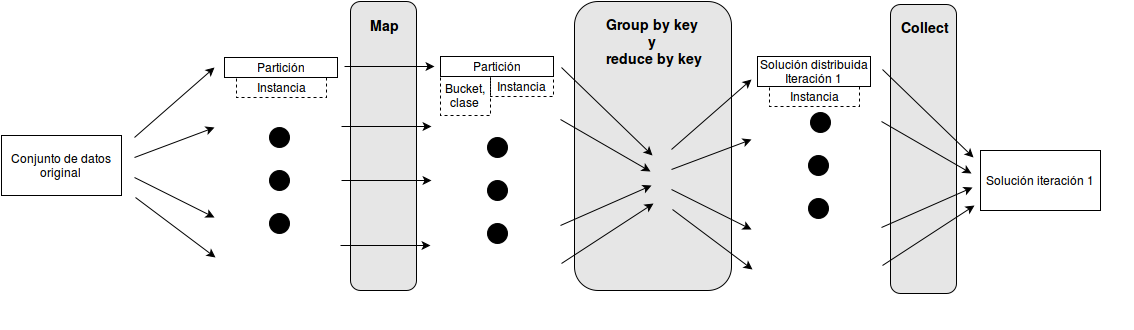
\includegraphics[width=1.0\textwidth]{img/memoria/diagram_LSHIS1}
		\caption{Diagrama de la ejecución del algoritmo LSHIS durante su primera iteración.}\label{fig:img/memoria/diagram_LSHIS1}
	\end{figure}
	\FloatBarrier
	
		\begin{figure}[!h]
		\centering
		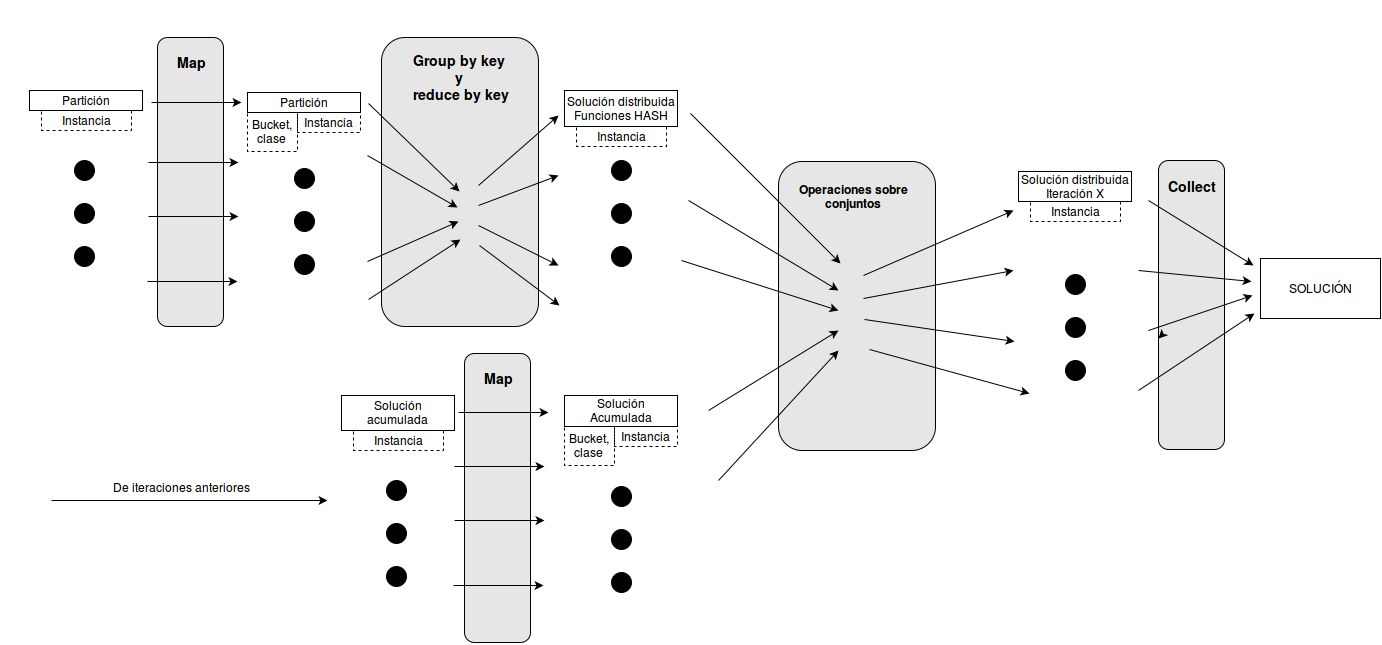
\includegraphics[width=1.0\textwidth]{img/memoria/diagram_LSHIS2}
		\caption{Diagrama de la ejecución del algoritmo LSHIS durante su segunda o mayor iteración.}\label{fig:img/memoria/diagram_LSHIS2}
	\end{figure}
	\FloatBarrier

%\imagen{img/memoria/diagram_LSHIS1}{Diagrama de la ejecución del algoritmo LSHIS durante su primera iteración.}
%\imagen{img/memoria/diagram_LSHIS2}{Diagrama de la ejecución del algoritmo LSHIS durante su segunda o mayor iteración.}


\subsection{Implementación concreta de DemoIS}

La implementación de este algoritmo no ha requerido modificar el pseudocódigo del mismo (ver \ref{sec:defDemoIS}) pero sí existen varios detalles que conviene destacar sobre la actual implementación.

En primer lugar, como puede apreciarse en la figura \ref{fig:img/memoria/diagram_DemoIS}, no todo el algoritmo se ejecuta en paralelo. A la hora de calcular el \textit{fitness} óptimo lo hacemos de manera secuencial. Esto es así porque no contamos con una implementación paralela del algoritmo KNN, necesario para este proceso (ver \ref{sec:ImplRecursosAdicionales}). Aún con esto, durante esa etapa del proceso solo seleccionamos un pequeño grupo de instancias en comparación con el conjunto inicial, por lo que operar con tal número de datos no supone un problema de rendimiento tan grande.

Existen otras consideraciones de cara a la implementación, como el uso de un particionador aleatorio que no genera particiones del mismo tamaño o la creación de una clase individual que evite la serialización completa del algoritmo al realizar la primera operación \textit{map}. Sin embargo, estos temas serán tratados con más detenimiento en el anexo incluido junto con la memoria.

%En segundo lugar, el particionado del conjunto de datos inicial para realizar las votaciones es aleatorio y genera particiones que no son estrictamente del mismo tamaño, sino que presentan ligeras variaciones de unas a otras. Esto es así porque, en un entorno paralelo, es muy complicado redistribuir las instancias entre los nodos de manera aleatoria pero, a la vez, generando particiones de tamaño similar (y, es por ello, que Spark no proporciona ningún tipo de clase o ayuda en este aspecto). Dado que estos algoritmos están pensados para su ejecución con un número muy grande de instancias, se confía en que la aleatoriedad sitúe un número muy similar de instancias en cada una de las particiones.

	\begin{figure}[!h]
		\centering
		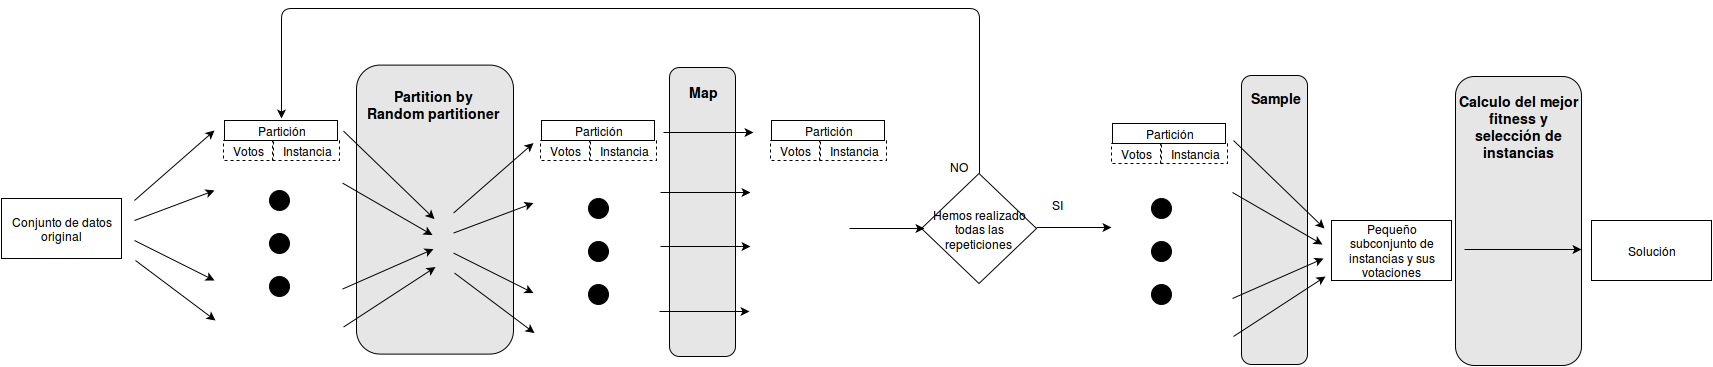
\includegraphics[width=1.0\textwidth]{img/memoria/diagram_DemoIS}
		\caption{Diagrama de la ejecución del algoritmo DemoIS.}\label{fig:img/memoria/diagram_DemoIS}
	\end{figure}
	\FloatBarrier

%\imagen{img/memoria/diagram_DemoIS}{Diagrama de la ejecución del algoritmo DemoIS.}

\section{Comparativa entre las implementaciones de Weka y Spark}

Como otro de los objetivos principales del proyecto, se procedió a realizar una comparación entre nuestras implementaciones de los algoritmos de selección de instancias con las ya existentes para su uso en Weka.

De nuevo, la finalidad de esta comparación tenía varios objetivos: evaluar el rendimiento entre ambas aproximaciones, comprobar el correcto funcionamiento de los algoritmos y evaluar como los cambios de implementación podían haber afectado a su funcionalidad.

Existe una sección más detallada donde se profundizará sobre todos los aspectos relacionados con la comparativa en la sección...

\todo{Incluir sección donde comparar los algoritmos de selección de instancias.}

\section{Implementación de un entorno gráfico}

En la etapa final, se vio como el proyecto había alcanzado una complejidad considerable en cuando a las opciones de lanzamiento se refiere. Este hecho hacía de la ejecución por línea de comandos un método de lanzamiento mucho más tedioso de lo que a un usuario normal podría resultarle ya de principio. Es por esta razón que, con la intención de facilitar el uso de la biblioteca, que se decidió la implementación de una pequeña interfaz gráfica que hiciese más intuitívo el uso del proyecto.

Así pues, se ha realizado una interfaz gráfica que permita introducir, mediante campos de texto, todas las opciones necesarias para la ejecución de los algoritmos, así como la posibilidad de seleccionar los diferentes conjuntos de datos o selectores de instancias. Además, posibilita la acción de crear baterías de ejecuciones al dar la opción de indicar más de una configuración de Spark, conjunto de datos y/o filtro a la vez.

Esta interfaz ofrece dos modos de ejecución:

\begin{itemize}
\item Permite ejecutar los algoritmos directamente desde la interfaz gráfica. Es una opción no recomendada si lo que se busca es eficiencia en los tiempos de ejecución pero es una manera sencilla de realizar pruebas sobre conjuntos de datos pequeños
\item Permite la compresión en un archivo de extensión .zip de todos los conjuntos de datos necesarios para llevar a cabo las ejecuciones y de un archivo .sh generado dinámicamente que permita la ejecución de todas las ejecuciones seleccionadas. Este tipo de operación facilita que el usuario pueda definir todas las operaciones desde su máquina y, posteriormente, pueda trasladarlas de manera sencilla a un servidor más potente donde serán ejecutadas.
\end{itemize}

\todo{Podría meterse la evolución de los prototipos aquí.}
\todo{Meter foto}




\begin{comment}
\section{Comparativa entre las ejecución de clasificadores en Weka y Spark}


Para realizar las mediciones utilizaremos conjuntos de datos de diferentes tamaños (detallados en la sección \ref{Datasets}), pero siempre un mismo algoritmo: el Naive Bayes. Naive Bayes es un algoritmo de clasificación probabilístico y relativamente simple que ya se encontraba implementado tanto en la librería de Weka como en la de Spark, razón por la cual ha sido elegido. En un principio hemos supuesto que no habría grandes diferencias en cuanto a tiempo de ejecución o recursos entre ambas implementaciones.

La ejecución del algoritmo se analizará tanto en Weka como en Spark, siendo en este último ejecutado con diferente número de hilos: 1, 2 y 4.

El programa utilizado para medir el rendimiento ha sido JConsole (ver \ref{DefJConsole}) en ambos casos, con el fin de utilizar la misma herramienta de monitorización en todos los experimientos.
Para observar el comportamiento de los hilos hemos utilizado la herramienta JvisualVM. (ver \ref{DefJvisualVM})

\subsection{Criterios comparados}

Los aspectos que hemos tenido en cuenta a la hora de recoger datos han sido:

\begin{itemize}
	\item \textbf{Tiempo de ejecución:} El periodo analizado es aquel que incluye la lectura de datos, la preparación, entrenamiento y prueba de los diferentes clasificadores que genere la validación cruzada y el cálculo del resultado final. Esta manera de medir es algo que afecta esencialmente a Spark, que lanza un gran número de procesos al iniciarse y pierde algo de tiempo con respecto a Weka.
	\item \textbf{Memoria:} Media del espacio de memoria RAM que consume la ejecución del algoritmo.
	\item \textbf{Porcentaje de CPU:} Media del porcentaje de CPU utilizado con respecto a la potencia total de la CPU. Estas pruebas han sido realizadas sobre una máquina con capacidad para soportar 4 hilos al mismo tiempo, por lo que el uso completo de uno de los hilos supondría un porcentaje de carga de la CPU del 25\% con respecto al total, el uso exclusivo de dos hilos sería un 50\% y así sucesivamente.
	\item \textbf{Comportamiento de los hilos:} Como actúan los hilos del programa cuando se ejecuta el clasificador. Al ser un elemento que no puede medirse directamente, se recurrirá a hablar de él en la sección \ref{ConclusionesWekaSpark} para sustentar otros argumentos, incluyendo imágenes que muestren el comportamiento en el caso de necesitarlas.
\end{itemize}

\todo{Las palabras "Media" aparecen subrayadas, no se por qué}

\subsection{Entorno de las pruebas}

Las mediciones se han llevado a cabo bajo las siguientes circunstancias:

\begin{itemize}
	\item Las ejecuciones se realizaron desde la terminal, tanto en el caso de Weka como en el de Spark.
	\item En todas las ejecuciones hemos contado con memoria suficiente como para poder incluir en ella todo el conjunto de datos. Es necesario destacar que, pese a todo, este supuesto no es común dentro de la minería de datos..
	\item Se necesita un tiempo para indicar a la herramienta de monitorización qué proceso ha de medir. Por ello, con la intención de tener tiempo para asociar la herramienta de monitorización al proceso concreto, la ejecución hilo principal es suspendida durante un pequeño periodo de tiempo antes de iniciar siquiera la lectura de datos del fichero.
	\item Aunque no estamos interesados en la salida final del algoritmo, queremos simular que se realizan las fases de validación y test. No se ha utilizado un archivo diferente como conjunto de test, sino que hemos utilizado una validación cruzada de 10 iteraciones.
	\item El formato utilizado en los ficheros que contienen datos ha sido .arff para Weka y .csv para Spark. La razón por la que no se han utilizado ficheros .csv en Weka ha sido por la posibilidad de que esto produzca errores a la hora de leer el archivo~\cite{CSVWeka}.
	\item El formato de los datos de los conjuntos de datos también ha sufrido variaciones. Mientras que los archivos .arff utilizados por Weka contienen los datos tal y como los proporciona el data set original, algunos conjuntos de datos han tenido que ser normalizados al transformarlos a .csv para poder ser utilizados en Spark. La razón es que el algoritmo NaiveBayes implementado en Spark no admite atributos negativos. Ha afectado a los conjuntos de datos ``Human Activity Recognition'', ``Covertype'' y ``HIGGS''(ver \ref{Datasets}) 
	\item En lo que se refiere a Spark, se ha creado objeto en Scala que es capaz de leer el conjunto de datos, crear diferentes \textit{folds} de dicho conjunto, entrenar y probar el clasificador y mostrar un resultado final. Weka ya proporciona herramientas de este tipo y por lo tanto no ha sido necesario generar ninguna otra clase.
	
\end{itemize}

\todo{Si se puede, se debería indicar el periodo que pasa entre las mediciones de RAM y de CPU}

\subsection{Conjuntos de datos}\label{Datasets}

Los conjuntos de datos, ordenados de menor a mayor según los recursos utilizados para correr el programa, han sido los siguientes:

\tablaSmall{Conjuntos de datos utilizados para la comparación entre Weka y Spark.}{m{5.55cm} >{\raggedleft\let\newline\\\arraybackslash\hspace{0pt}}m{2.35cm} m{2.35cm} m{2.35cm}}{ConjuntosWekaSpark}
{\centering Nombre del conjunto & \centering Instancias & \centering Atributos  & \multicolumn{1}{c}{Clases} \\}{

\centering Iris & 150 & \centering 4 & \multicolumn{1}{c}{3}  \\ [0.2cm]
\centering Human Activity Recognition \cite{HumanActivityDataset} & 165.632 & \centering 17 & \multicolumn{1}{c}{5}   \\ [0.2cm]
\centering Poker \cite{Lichman:2013} & 1.025.010 & \centering 10 & \multicolumn{1}{c}{10}  \\ [0.2cm]
\centering Covertype \cite{Lichman:2013} & 581.012 & \centering 54 & \multicolumn{1}{c}{6}  \\ [0.2cm]
\centering HIGGS \cite{Lichman:2013} \cite{HIGGSDataSet} & 1.469.873 y 2.939.746\tablefootnote{El conjunto original consta de 11.000.000 instancias, pero he reducido su tamaño original para acercarlo más al tamaño de los otros conjuntos.} & \centering 28 & \multicolumn{1}{c}{2} \\ [0.2cm]

} 
\todo{Revisar el código de la tabla}

Indicar que, a la hora de seleccionar los conjuntos, se han elegido aquellos que compartan algunas características comunes:

\begin{itemize}
	\item No existen campos de tipo texto. La única excepción la encontramos en los atributos de clase en los ficheros .arff, pero estos atributos serán tratados como nominales a la hora de la clasificación en Weka.
	\item No existen campos vacíos en ninguna de las instancias de los atributos.
\end{itemize}

\subsection{Resultados}

Los resultados obtenidos han sido agrupados según el conjunto de datos utilizado.

Las pruebas han sido ejecutadas bajo una validación cruzada de 10 x 2, de manera que podamos comprobar si el resultado obtenido se encuentra dentro de lo esperado o su buen/mal funcionamiento se debe a una circunstancia puntual. 

\todo{Replantear tablas de resultados. Crear una sola tabla}

\tablaSmall{Rendimiento sobre el conjunto de datos Iris.}{l c c c c}{RendimientoIris}
{\multicolumn{1}{c}{Criterio} & Weka & Spark 1 hilo & Spark 2 hilos  & Spark 4 hilos \\}{

 Tiempo (s) & 0,1 & 1,97 & 2,13 & 2,15 \\ [0.2cm]
 Memoria (MB)\tablefootnote{\label{noteIris}Los datos de las mediciones sobre el uso de memoria y CPU en el conjunto Iris no son concluyentes debido al corto periodo de tiempo que tardan en ejecutarse.} & - & - & - & - \\ [0.2cm]
 CPU (\%)\footref{noteIris} & - & - & - & - \\ [0.2cm]

}

\tablaSmall{Rendimiento sobre el conjunto de datos Human Activity Recognition.}{l c c c c}{RendimientoHAR}
{\multicolumn{1}{c}{Criterio} & Weka & Spark 1 hilo & Spark 2 hilos  & Spark 4 hilos \\}{

 Tiempo (s) & 12,37 & 16,13 & 11,75 & 11,71 \\ [0.2cm]
 Memoria (MB) & 242,01 & 173,80 & 219,75 & 219,17 \\ [0.2cm]
 CPU (\%) & 25,5 & 36,02 & 54,03 & 59,43\\ [0.2cm]

}

\tablaSmall{Rendimiento sobre el conjunto de datos Poker.}{l c c c c}{RendimientoPoker}
{\multicolumn{1}{c}{Criterio} & Weka & Spark 1 hilo & Spark 2 hilos  & Spark 4 hilos \\}{

 Tiempo (s) & 73,90 & 47,44 & 31,84 & 30,77  \\ [0.2cm]
 Memoria (MB) & 424,65 & 162,93 & 243,76 & 255,11\\ [0.2cm]
 CPU (\%) & 30,05 & 29,41 & 51,22 & 55,68 \\ [0.2cm]

}

\tablaSmall{Rendimiento sobre el conjunto de datos Covertype.}{l c c c c}{RendimientoCovertype}
{\multicolumn{1}{c}{Criterio} & Weka & Spark 1 hilo & Spark 2 hilos  & Spark 4 hilos \\}{

 Tiempo (s) & 183,95 & 101,91 & 73,23 & 53,78 \\ [0.2cm]
 Memoria (MB) & 576,78 & 177,37 & 213,7 & 211,7\\ [0.2cm]
 CPU (\%) & 28,17 & 28,26 & 43,10 & 71,94 \\ [0.2cm]

}

\tablaSmall{Rendimiento sobre el conjunto de datos HIGGS (1.469.873 instancias).}{l c c c c}{RendimientoHIGGS1}
{\multicolumn{1}{c}{Criterio} & Weka & Spark 1 hilo & Spark 2 hilos  & Spark 4 hilos \\}{

 Tiempo (s) & 246,97 & 191,9 & 130,37 & 99,2 \\ [0.2cm]
 Memoria (MB) & 832,88 & 872,56 & 864,92 & 921,49 \\ [0.2cm]
 CPU (\%) & 28,60 & 26,64 & 49,91 & 89,24\\ [0.2cm]

}

\tablaSmall{Rendimiento sobre el conjunto de datos HIGGS (2.939.746 instancias).}{l c c c c}{RendimientoHIGGS2}
{\multicolumn{1}{c}{Criterio} & Weka & Spark 1 hilo & Spark 2 hilos  & Spark 4 hilos \\}{

 Tiempo (s) & 503,929 & 368,721 & 264,023 & 215,214\\ [0.2cm]
 Memoria (MB) & 1747,22  & 883,28 & 911,77 & 853,58 \\ [0.2cm]
 CPU (\%) & 29 & 26,37 & 50,74 & 91,58 \\ [0.2cm]

}

\subsection{Conclusiones}\label{ConclusionesWekaSpark}
\todo{¿Mover esta sección al final de la memoria?}
\todo{Revisar las referencias ante un cambio de tabla de resultados.}
\begin{itemize}
	\item Puede observarse claramente que Weka es considerablemente superior a Spark cuando utilizamos conjuntos de datos pequeños, como observamos en la tabla \ref{tabla:RendimientoIris} o incluso en la tabla \ref{tabla:RendimientoHAR}, pero su rendimiento se ve superado con notable diferencia cuando el conjunto de datos empieza a sobrepasar las 100.000 instancias de Human Activity Recognition (ver \ref{Datasets}).
	\item Salvo cuando tratamos con conjuntos de datos pequeños, vease por ejemplo la tabla \ref{tabla:RendimientoIris}, el rendimiento del algoritmos Naive Bayes de Weka es menor si lo comparamos con las ejecuciones sobre un solo hilo de Naive Bayes en Spark. Es posible que una de las causas sea la diferente implementación del algoritmo en Weka y en Spark.
	\item Como era de esperar, doblar el número de hilos no implica reducir a la mitad el tiempo de procesamiento, sino que genera un beneficio menor que, en algún momento y dependiendo del tamaño del conjunto de datos analizado, dejará de ser significativo aunque sigamos añadiendo hilos.
	\missingfigure{Probablemente incluya una gráfica sobre el rendimiento de Spark sobre HIGGS}
	\item Generalmente Spark necesita menos memoria que Weka para ejecutar el programa.
	\item Parece que el porcentaje de RAM requerido por Spark aumenta ligeramente cuantos más hilos tengamos en ejecución, algo que se aprecia bien en los conjuntos de datos pequeños.
	\item El porcentaje de uso de la CPU en Weka se situa siempre entorno a los valores 25-30\%. Esto es así porque la ejecución de todas las tareas es lineal, consumiendo únicamente un hilo de los 4 que posee la máquina en la que se están realizando las prueba.
	\item Vemos que el porcentaje de uso de la CPU en las diferentes pruebas con Spark suele corresponder al número de hilos con los que se lanza la aplicación: 25\% para un hilo, 50\% para dos y, teóricamente, 90-100\% para 4. Sin embargo, y como podemos apreciar en las tablas \ref{tabla:RendimientoPoker} o \ref{tabla:RendimientoCovertype}, la ejecución con cuatro hilos no aprovecha al máximo las capacidades del procesador cuando el conjunto de datos es pequeño. Observando más de cerca el evento, vemos que, independientemente del número de hilos que decimos a Spark que maneje, en estos conjuntos de datos únicamente se lanzan dos hilos como máximo. Atribuimos esto a un comportamiento propio de Spark, que evalua que no existe necesidad de manejar tantos hilos de ejecución. 
	\missingfigure{Incluir comportamiento de los hilos de jvisualvm}
\end{itemize}


\section{Comparativa entre la ejecución del algoritmo LSHIS en Spark y Weka}

\subsection{Criterios comparados}

Se ha realizado la comparación teniendo en mente la medición de los siguientes parámetros:

\begin{itemize}
	\item \textbf{Reducción del conjunto de datos:} Relación entre el tamaño del conjunto de datos original y el obtenido tras la aplicación del algoritmo.
	\item \textbf{Tiempo de ejecución:} Tiempo real que ha requerido la ejecución del algoritmo LSHIS.
	\item \textbf{Precisión de un clasificador con el nuevo conjunto:} Porcentaje de acierto en test al aplicar el algoritmo KNN (K-Nearest neighbors) sobre el nuevo conjunto de datos.
\end{itemize}
\subsection{Entorno de las pruebas}
\begin{itemize}
	\item Las pruebas han sido ejecutadas bajo una validación cruzada de 10 x 2. \todo{ En la comparación de arriba esto está en otro sitio.}
		\item Todos los conjuntos de datos han sido normalizados
\end{itemize}

\subsection{Conjuntos de datos}

\todo{Esto ya esta arriba}

\subsection{Resultados}

\tablaSmall{Comparativa de LSHIS sobre el conjunto de datos Iris.}{l c c c c}{CompIrisLSHIS}
{\multicolumn{1}{c}{Criterio} & Weka & Spark 1 Ejecutor & Spark 2 Ejecutores  & Spark 4 Ejecutores \\}{

 Instancias & 22 & 26 & 23 & 22 \\ [0.2cm]
 Tiempo(s) & 12 & 3340 & 2670 & 10574 \\ [0.2cm]
 Acierto(\%) & 92 & - & - & - \\ [0.2cm]

}

\tablaSmall{Comparativa de LSHIS sobre el conjunto de datos Human Activity.}{l c c c c}{CompHALSHIS}
{\multicolumn{1}{c}{Criterio} & Weka & Spark 1 Ejecutor & Spark 2 Ejecutores  & Spark 4 Ejecutores \\}{

 Instancias & 147 & 350 & 340 & 367 \\ [0.2cm]
 Tiempo(s) & 167 & 9919 & 12327 & 22525 \\ [0.2cm]
 Acierto(\%) & 57,1 & 71,95 & 69,21 & 69,4 \\ [0.2cm]

}


\tablaSmall{Comparativa de LSHIS sobre el conjunto de datos Poker.}{l c c c c}{CompPokerLSHIS}
{\multicolumn{1}{c}{Criterio} & Weka & Spark 1 Ejecutor & Spark 2 Ejecutores  & Spark 4 Ejecutores \\}{

 Instancias & 3806 & 7545 & 7613 & 7625 \\ [0.2cm]
 Tiempo(s) & 823 & 24057 & 19448 & 26464 \\ [0.2cm]
 Acierto(\%) & 26,13 & 27,14 & 31,26 & 30,62 \\ [0.2cm]

}


\tablaSmall{Comparativa de LSHIS sobre el conjunto de datos Covertype.}{l c c c c}{CompCovLSHIS}
{\multicolumn{1}{c}{Criterio} & Weka & Spark 1 Ejecutor & Spark 2 Ejecutores  & Spark 4 Ejecutores \\}{

 Instancias & 2317 & 3987 & 3969 & 3982 \\ [0.2cm]
 Tiempo(s) & 570 & 24527 & 22157 & 27262 \\ [0.2cm]
 Acierto(\%) &  &  &  &  \\ [0.2cm]

}

\tablaSmall{Comparativa de LSHIS sobre el conjunto de datos HIGGS. (1.469.873 instancias)}{l c c c c}{CompHIGGS1LSHIS}
{\multicolumn{1}{c}{Criterio} & Weka & Spark 1 Ejecutor & Spark 2 Ejecutores  & Spark 4 Ejecutores \\}{

 Instancias &  &  &  &  \\ [0.2cm]
 Tiempo(s) &  &  &  &  \\ [0.2cm]
 Acierto(\%) &  &  &  &  \\ [0.2cm]

}

\tablaSmall{Comparativa de LSHIS sobre el conjunto de datos HIGGS. (2.939.746 instancias)}{l c c c c}{CompHIGGS2LSHIS}
{\multicolumn{1}{c}{Criterio} & Weka & Spark 1 Ejecutor & Spark 2 Ejecutores  & Spark 4 Ejecutores \\}{

 Instancias &  &  &  &  \\ [0.2cm]
 Tiempo(s) &  &  &  &  \\ [0.2cm]
 Acierto(\%) &  &  &  &  \\ [0.2cm]

}



\subsection{Conclusiones}

\begin{itemize}
	\item No se puede predecir la salida de Spark por ser la ejecución en paralelo.
	\item Con tan poca carga de trabajo, Weka es mucho mejor. A partir de Poker podemos ver que Spark empieza a funcionar un poco como debería, donde 2 ejecutores funcionan mejor que 1, pero nunca llegamos a necesitar los 4 cores.
	\item
\end{itemize}


\end{comment}